\documentclass[tikz]{standalone}

\usetikzlibrary{angles}

\colorlet{FilledSurface}{blue!20}
\colorlet{FilledSurfaceGroupOne}{blue!20}
\colorlet{FilledSurfaceGroupTwo}{red!20}
\colorlet{FilledSurfaceGroupThree}{green!20}
\colorlet{FilledSurfaceGroupFour}{magenta!20}
\colorlet{FormulaBackground}{green!10}
\colorlet{FormulaFrame}{green}

\usetikzlibrary{calc}

\begin{document}
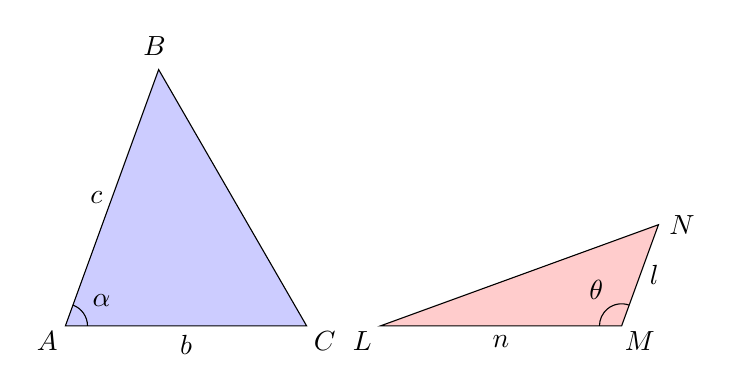
\begin{tikzpicture}

    \def\offset{0.3}

    % Triángulo 1

    \def\tOneCircumradius{2}
    \def\tOneAngleA{220}
    \def\tOneAngleB{100}
    \def\tOneAngleC{320}

    \coordinate (tOneCenter) at (0, 0);
    \path[overlay] (tOneCenter) circle (\tOneCircumradius);
    \coordinate (tOneA) at (\tOneAngleA:\tOneCircumradius);
    \coordinate (tOneB) at (\tOneAngleB:\tOneCircumradius);
    \coordinate (tOneC) at (\tOneAngleC:\tOneCircumradius);
    \draw[fill=FilledSurfaceGroupOne]
    (tOneA) -- node [left] {$c$}
    (tOneB) --
    (tOneC) -- node [below] {$b$}
    cycle;

    \node at ($(tOneCenter) + (\tOneAngleA:\tOneCircumradius + \offset)$) {$A$};
    \node at ($(tOneCenter) + (\tOneAngleB:\tOneCircumradius + \offset)$) {$B$};
    \node at ($(tOneCenter) + (\tOneAngleC:\tOneCircumradius + \offset)$) {$C$};

    % Triángulo 2

    \def\tTwoCircumradius{2}
    \def\tTwoAngleL{220}
    \def\tTwoAngleN{0}
    \def\tTwoAngleM{320}

    \coordinate (tTwoCenter) at (4, 0);
    \path[overlay] (tTwoCenter) circle (\tTwoCircumradius);
    \coordinate (tTwoL) at ($(tTwoCenter) + (\tTwoAngleL:\tTwoCircumradius)$);
    \coordinate (tTwoN) at ($(tTwoCenter) + (\tTwoAngleN:\tTwoCircumradius)$);
    \coordinate (tTwoM) at ($(tTwoCenter) + (\tTwoAngleM:\tTwoCircumradius)$);
    \draw[fill=FilledSurfaceGroupTwo]
    (tTwoL) --
    (tTwoN) -- node [right] {$l$}
    (tTwoM) -- node [below] {$n$}
    cycle;

    \node at ($(tTwoCenter) + (\tTwoAngleL:\tTwoCircumradius + \offset)$) {$L$};
    \node at ($(tTwoCenter) + (\tTwoAngleN:\tTwoCircumradius + \offset)$) {$N$};
    \node at ($(tTwoCenter) + (\tTwoAngleM:\tTwoCircumradius + \offset)$) {$M$};

    \path pic [draw, angle radius = 8pt, angle eccentricity = 2pt, pic text={$\alpha$}] {angle = tOneC--tOneA--tOneB};
    \path pic [draw, angle radius = 8pt, angle eccentricity = 2pt, pic text={$\theta$}] {angle = tTwoN--tTwoM--tTwoL};

\end{tikzpicture}
\end{document}


